\section{Electron Identification}\label{sec:electronID}
\subsection{Offline object reconstruction and identification}\label{subsec:electron_offline}


The offline reconstruction of electrons and photons~\cite{ATLAS-EGAM-2018-01} is based on dynamic, variable-sized clusters of energy deposits, known as topo-clusters, formed from topologically connected electromagnetic (EM) and hadronic calorimeter cells~\cite{PERF-2014-07}. These clusters help to recover
energy lost due to bremsstrahlung photons or electrons originating from photon conversions. After applying initial corrections for position and energy calibration, the topo-clusters are matched to tracks in the ID that have been re-fitted to account for bremsstrahlung effects,
following the method outlined in Ref.~\cite{ATLAS-CONF-2012-047}, to reconstruct electron candidates. Topo-clusters that are either unmatched to any track or matched to a track associated to a conversion vertex are reconstructed as photon candidates. Once candidates are formed, their energies undergo further recalibration for use in analyses.

Prompt electrons traversing the central region of the detector ($|\eta| < 2.47$) are identified using a likelihood-based (LH) method, which uses several discriminating variables: the longitudinal and lateral shapes of EM showers, the quality of the track, matching criteria between track and cluster,
and particle identification information from the TRT. The probability density functions (pdfs) used in the LH approach are derived from $J/\psi\rightarrow ee$ decays for the transverse energy (\et{}) range of 4.5--15~\GeV{}, and from $Z\rightarrow ee$ decays for \et$\,>15$~\GeV{}, as detailed in~\cite{ATLAS-EGAM-2018-01}. Separate pdfs are defined for each discriminant variable across different bins of \et{} and $\eta$ of the electron-candidate.

%To maintain a smooth electron identification efficiency as a function of \et{}, the LH discriminant thresholds
%are adjusted within finer \et{} bins than those used for the pdfs. At the boundaries between \et{} bins,
%a linear interpolation of both the pdfs and the discriminant thresholds is applied, a method referred to as
%`smoothing'. Additionally, the discriminant threshold is varied linearly with the number of reconstructed
%primary vertices to ensure consistent rejection of background electrons.

Three identification operating points (called ``loose'', ``medium'' and ``tight'') are defined, each corresponding to progressively tighter requirements on the LH discriminant. The average efficiencies for electrons from electroweak processes (evaluated over the
2015--2017 dataset) are approximately: 93\% (loose), 88\% (medium), and 80\% (tight).


\subsection{Online reconstruction and identification at trigger level}\label{subsec:electron_online}

Electron reconstruction at the HLT stage is performed on each EM RoI provided by L1, which satisfies $E_T$ and isolation requirements as specified by the trigger configuration. It proceeds in a series of sequential steps as shown in the schematic diagram in Figure~\ref{fig:electron_chain}.  Lozenges represent feature-extracting algorithms that are responsible for building electron properties from detector data (calorimeter shower shapes, transverse momentum, energy, position, etc.). Rectangles represent hypothesis-testing algorithms, which apply selection requirements on those reconstructed properties. % e uses these attributes to decide if the incoming particle is an electron or a jet.


\begin{figure}[h!tb]
  \centering
  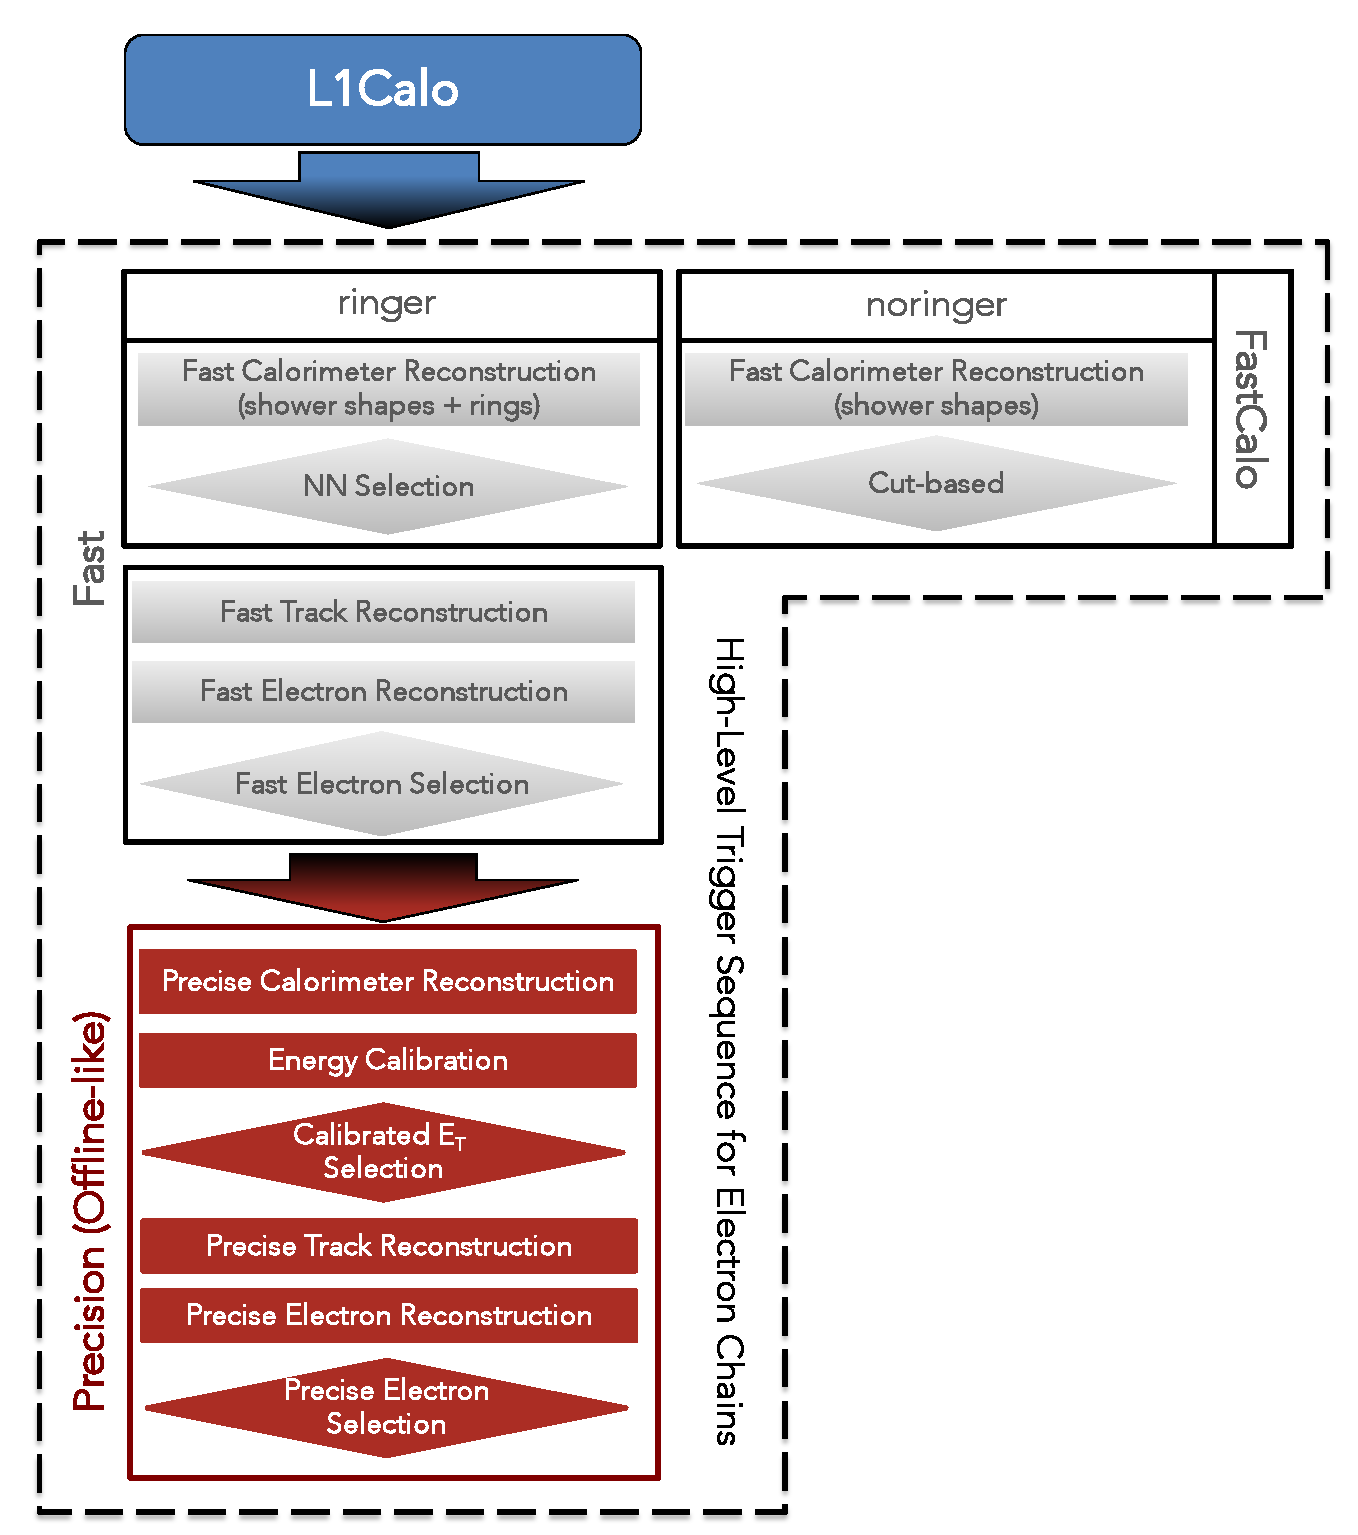
\includegraphics[width=0.7\textwidth]{figures/ElectronChain_Run2_noringer_and_ringer.pdf}
  \caption{Diagram of the sequence of algorithms used to select electron candidates at the High Level Trigger stage. Differences between the original baseline (no-ringer) and ringer-based electron triggers lie in the first step, called FastCalo. Grey blocks represent algorithms in the fast stage, and red blocks represent precision-step algorithms.}
  \label{fig:electron_chain}
\end{figure}

Electron identification at the HLT selection begins with a fast calorimeter reconstruction (FastCalo) step, which has two implementations: the original/baseline cut-based selection and the novel neural-network (NN) approach using the Neural-Ringer algorithm presented in this paper. The latter is implemented for triggering electrons with ET $\geq$ 15 GeV. FastCalo is followed by a fast tracking-reconstruction step, which builds tracks for electron candidates only inside the RoI. A fast electron hypothesis algorithm applies identification requirements by combining the results of both fast algorithms. Reconstruction algorithms are then executed for trigger electron candidates satisfying the fast electron hypothesis selection. 
%on both fast algorithms If a particle candidate satisfies the criteria defined for the fast electron selection, the precision algorithms are executed in the HLT, where access to detector information outside the RoI is possible. These precision online algorithms are similar to their offline counterparts. 

In the precision calorimeter reconstruction step, the cluster reconstruction and calibration are similar to those for photons, and to those used offline in early Run 2 analyses \cite{PERF-2017-01}. Then, ID tracks within the
RoI are extrapolated to the second layer of the EM calorimeter and are required to match the electron candidate cluster within $|\Delta\eta(\text{track, cluster})| < 0.05$ and $|\Delta\phi\text{(track, cluster)}| < 0.05$ rad.
The precision electron selection combines the results of the precision calorimeter and precision tracking steps to build a likelihood (LH) discriminant with four operating points: ``lhvloose'', ``lhloose'', ``lhmedium'', and ``lhtight''. The identification in the trigger is designed to be as close as possible to the offline version, except for the following differences: 
the discriminating variables used online have different resolutions; 
the momentum loss due to bremsstrahlung, $\Delta p/p$, is not accounted for in the online LH.  

An important aspect for trigger operation is the amount of simultaneous particle interactions in the detector ($\mu$), which generates pileup of events in the electronics readout system and may change the typical energy deposition profile in the calorimeters for electromagnetic particles. The online selection uses an estimate of \avgmu{}, the mean number of collisions during a reference period, to measure pileup instead of the number of primary vertices used offline. % \footnote{an overlap of multiple proton-proton collisions within the detector, resulting in a superposition of particle signals in the same LHC bunch-crossing.} and adjust the discriminant threshold requirement. 
%some discriminating variables used in offline selection are not present in online version due to CPU constraints.

%Triggers with ‘nod0’ suffixed to their name do not include the transverse impact parameter relative to the beam-line, $d_0$, and its significance, in the online LH version. 

An additional, optional requirement of isolation denoted ‘ivarloose’ is also available for electron triggers. This tracking-only isolation is required to satisfy 
$p_T^{iso}(\Delta R^{var}<0.2)/p_T < 0.10$ and is calculated similarly to the offline isolation operating points.

